%
\section{Introduction}
\label{sec:intro}


\cxj{Is your goal reconstruction or building extraction? The introduction should explain the overall goal. What are the challenges for building modeling from remote sensing images? What kind of work has been done in the literature? Why do we focus on building detection? What are our contributions?}

\IEEEPARstart{B}{uilding} extraction, which aims to extract rooftop\footnote{Because the data sets used in our article are high altitude remote sensing images which could be considered as the top views of the ground. Therefore, we do not distinguish the concepts of buildings and rooftops in the subsequent description.} in a large-scale remote sensing image, remains one of the fundamental challenges have been studied for decades in the field of remote sensing. Moreover, auto extraction of building rooftops from aerial and satellite imagery is an important step in many applications, such as: urban planing, automated map making, 3D city modeling, updating geographical dataset and military reconnaissance. But, it is particularly difficult to extract rooftop at the pixel level for the following reasons:
\begin{itemize}
 \item Different density of buildings in the scene. A rural scene has low density but an urban scene has high density, with a suburban scene in between (medium density).
 \item Diverse shapes of the buildings. Buildings come in many shapes from simple rectangular blocks with flat roof to complex shapes with intricate roof shape.
 \item The quality of remote sensing images. Images vary in terms of contrast, resolution, and image principle \cite{IEEEexample:huertas1988detecting}.
\end{itemize}

 Several patches are shown in Fig.~\ref{fig:intro} \cxj{do not use the figure no directly. using ref{}..} , which illustrate the different challenges of building extraction task.


\begin{figure}
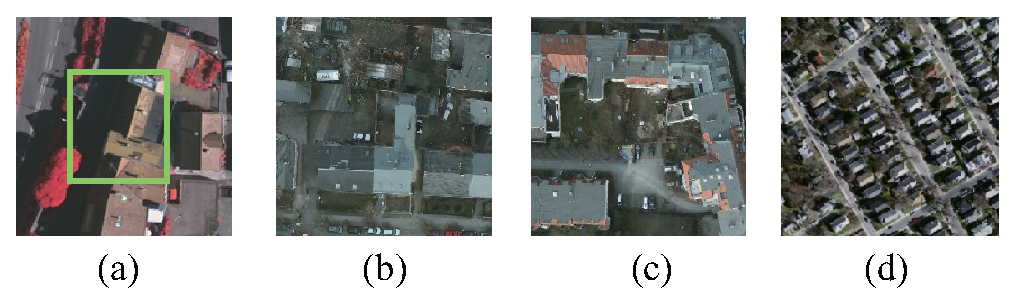
\includegraphics[width=8.7cm]{Figures/challenge.eps}
\caption{Examples of remote sensing patches with different kinds of challenges. (a) Shadow occlusion in green frame. (b) Low inter-class differences. (c) High intra class variance. (d) A lot of tiny buildings close to each other.}
\label{fig:intro}
\end{figure}


In the past decades, many researchers have made several effort to extract buildings automatically.
At first, many simple knowledge-based methods were put forward by \cite{IEEEexample:huertas1988detecting}, \cite{IEEEexample:noronha2001detection}, \cite{IEEEexample:nosrati2009novel}, \cite{IEEEexample:izadi2012three}, \cite{IEEEexample:wang2015efficient}.
Their basic ideas are derived from prior knowledge that buildings are closed polygons made up of some straight lines.
Some others are energy based methods including the variational level set evolution, improved snake model and graph cut \cite{IEEEexample:cote2013automatic}, \cite{IEEEexample:peng2005improved}, \cite{IEEEexample:sirmacek2009urban}. Due to early methods depend too much on prior and initialization. It does not apply to building extraction of complex scene.


In recent years, with the development of machine learning, many techniques via machine learning are gradually introduced into the remote sensing domain.
At first, some shallow networks were proposed for multiple geographic object extraction\cite{IEEEexample:mnih2013machine}, \cite{IEEEexample:saito2016multiple}, \cite{IEEEexample:alshehhi2017simultaneous},\cite{IEEEexample:zhao2017contextually}. Since methods use patches for segmentation, they are inefficient and inaccurate for the pixel-wise segmentation task.
Further, with the growth of computer power, deep learning developed rapidly and brought into the field of remote sensing. Some researchers tried deep learing for aerial images classification and semantic pixel labelling~\cite{IEEEexample:paisitkriangkrai2015effective}, \cite{IEEEexample:liu2017dense}, \cite{IEEEexample:audebert2017deep}, \cite{IEEEexample:kampffmeyer2017urban}, \cite{IEEEexample:he2017multi}. Unfortunately, owing to ignoring the hierarchical information extracted by the network, they could not deal with the case that scenes of close-packed buildings well.



To fix the above problems, a relatively simple, but very effective fusion operation is proposed in this work. And it could be combined into a general CNN architecture easily for building extraction. 
Differ from above mentioned methods, we take full advantages of the low-level appearance information as well as high-level semantic information by the novel fusion operation in a way of stage by stage.
Inspired by FCN\cite{IEEEexample:Long_2015_CVPR} whose output is in the same resolution of input, we propose a noval hierarchically fused FCN, named HF-FCN for buildings pixel-wise classification.
Differ from the traditional FCN, a set of hierarchical fusion operations are used to fuse the intra layer information and inter layer information respectively which improve the performance of FCN greatly.
And numerous experiments conducted on three remote sensing image datasets all obtain fairly good results.
Further, we extend our work to the field of 3D modeling as the part of building detection. It is easily intergrated into the pipeline of building reconstruction and achieve good performance.
Our technical contributions are:
%
\begin{enumerate}
	\item A effective hierarchical fusion operation which is specially designed for multi-scale building extraction is proposed. Combining with a general FCN, a novel network is presented, named HF-FCN that can deal with the problems of different sizes, diverse appearance and mutual occlusion of buildings and etc.
	\item HF-FCN is an end-to-end network that does not need any post processing. And the approach is significantly computationally efficient than existing techniques. Besides, the overall accuracy based on HF-FCN exceeds the state-of-art algorithms.
\end{enumerate}

The remainder of this paper is organized as follows. Sec.~\ref{Sec:RelatedWork} sums up the related works in the past.
In Sec.~\ref{Sec:HF-FCN}, we introduce the fusion operation and architecture of HF-FCN. The training loss are also presented.
And in Sec.~\ref{Sec:exp}, a brief description of the dataset used for our task is provided. HF-FCN training strategies, details and its evaluation metrics are also described.
In Sec.~\ref{Sec:Res}, we display and analysis the experimental results.
Extension in 3D building modeling are presented in Sec.~\ref{sec:app}.
Finally, the conclusion is discussed in Sec.~\ref{Sec:Con}.
